%!Tex Root = ../Tutorat6.tex
% ./Packete.tex
% ./Design.tex
% ./Deklarationen.tex
% ./Aufgabe1.tex
% ./Aufgabe3.tex

\section{Task 2}

\setcounter{task}{1}

\begin{frame}[allowframebreaks]{Task 2}{Integer Linear Programming}
  \begin{tasknoinc}
    \begin{columns}
      \begin{column}{.5\textwidth}
        \centering
        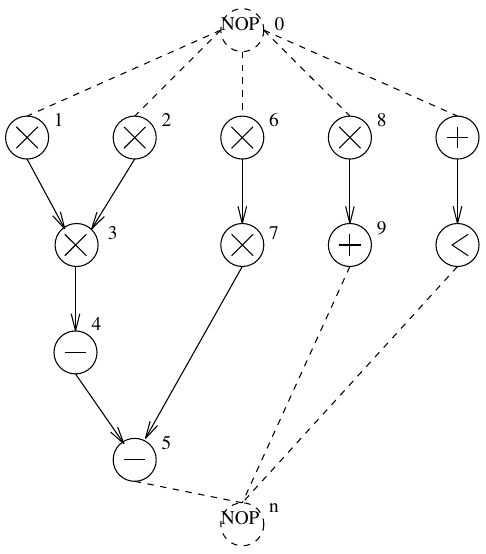
\includegraphics[height=.6\paperheight]{./figures/task2_sequence_graph.png}
      \end{column}
      \begin{column}{.5\textwidth}
        \begin{itemize}
          \item \alert{resource type $r_1$:} multiplication operation takes $2$ time units and $2$ units of this resource type are allocated
          \item \alert{resource type $r_2$:} all other ALU Operations take $1$ time unit and $2$ units of this resource type are allocated
        \end{itemize}
      \end{column}
    \end{columns}
  \end{tasknoinc}
  \begin{requirementsnoinc}
    \centering
    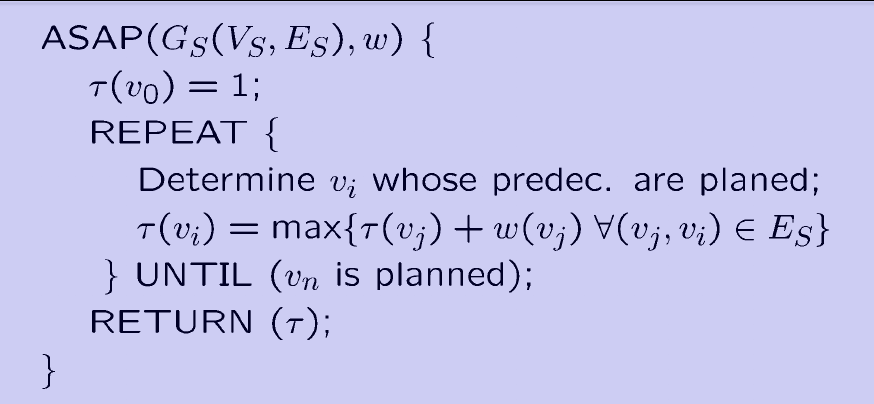
\includegraphics[width=0.6\textwidth]{./figures/asap.png}
  \end{requirementsnoinc}
  \begin{requirementsnoinc}
    \centering
    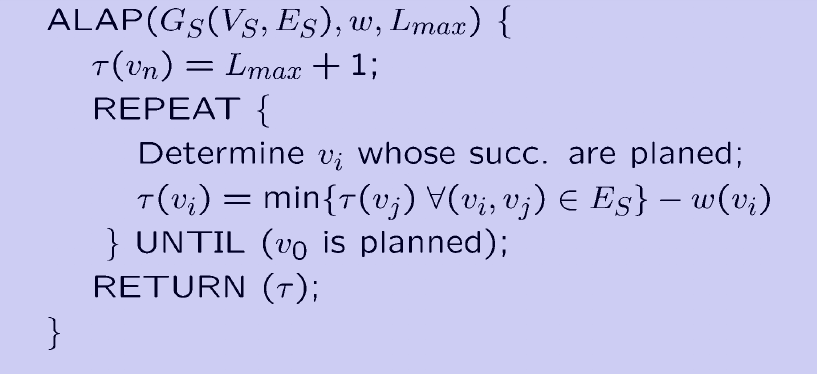
\includegraphics[width=0.6\textwidth]{./figures/alap.png}
  \end{requirementsnoinc}
  \begin{solutionnoinc}
    \centering
    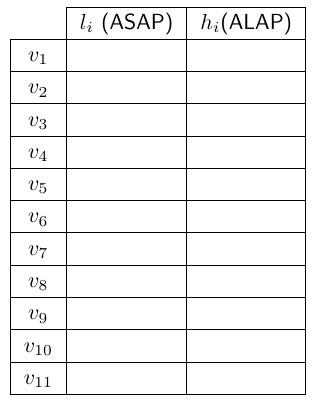
\includegraphics[height=0.6\paperheight]{./figures/task2_earliest_and_latest_starting_times_empty.png}
  \end{solutionnoinc}
  \begin{solution}
    \centering
    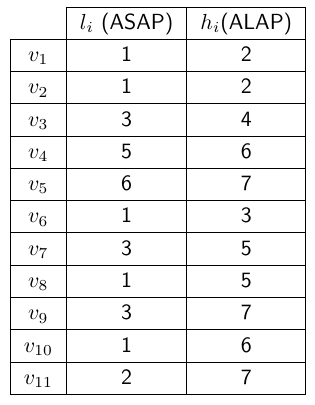
\includegraphics[height=0.6\paperheight]{./figures/task2_earliest_and_latest_starting_times.png}
  \end{solution}
  \begin{solutionnoinc}
    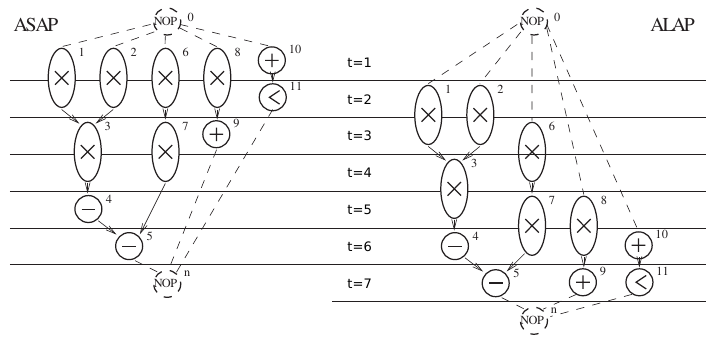
\includegraphics[width=\textwidth]{./figures/task2_scheduling_with_asap_and_alap.png}
  \end{solutionnoinc}
\end{frame}
\begin{frame}[allowframebreaks]{Task 2}{Integer Linear Programming}
  \begin{solutionnoinc}
    \begin{itemize}
      \item \alert{(i) Objective function:}
      \[
      \min \quad L=\tau\left(v_n\right)-\tau\left(v_0\right)
      \]
      \item \alert{(ii) Introduction of binary variables:}
      \[
        \begin{aligned}
        & x_{1,1}+x_{1,2}=1 \quad 1 \cdot x_{1,1}+2 \cdot x_{1,2}=\tau\left(v_1\right) \\
        & x_{2,1}+x_{2,2}=1 \quad 1 \cdot x_{2,1}+2 \cdot x_{2,2}=\tau\left(v_2\right) \\
        & x_{3,3}+x_{3,4}=1 \quad 3 \cdot x_{3,3}+4 \cdot x_{3,4}=\tau\left(v_3\right) \\
        & x_{4,5}+x_{4,6}=1 \quad 5 \cdot x_{4,5}+6 \cdot x_{4,6}=\tau\left(v_4\right) \\
        & x_{5,6}+x_{5,7}=1 \quad 6 \cdot x_{5,6}+7 \cdot x_{5,7}=\tau\left(v_5\right) \\
        \end{aligned}
      \]
    \end{itemize}
  \end{solutionnoinc}
  \framebreak
  \begin{solutionnoinc}
      \[
      \begin{aligned}
        & x_{6,1}+x_{6,2}+x_{6,3}=1 \quad 1 \cdot x_{6,1}+2 \cdot x_{6,2}+3 \cdot x_{6,3}=\tau\left(v_6\right) \\
        & x_{7,3}+x_{7,4}+x_{7,5}=1 \quad 3 \cdot x_{7,3}+4 \cdot x_{7,4}+5 \cdot x_{7,5}=\tau\left(v_7\right) \\
        & x_{8,1}+\ldots+x_{8,5}=1 \quad 1 \cdot x_{8,1}+\ldots+5 \cdot x_{8,5}=\tau\left(v_8\right) \\
        & x_{9,3}+\ldots+x_{9,7}=1 \quad 3 \cdot x_{9,3}+\ldots+7 \cdot x_{9,7}=\tau\left(v_9\right) \\
        & x_{10,1}+\ldots+x_{10,6}=1 \quad 1 \cdot x_{10,1}+\ldots+6 \cdot x_{10,6}=\tau\left(v_{10}\right) \\
        & x_{11,2}+\ldots+x_{11,7}=1 \quad 2 \cdot x_{11,2}+\ldots+7 \cdot x_{11,7}=\tau\left(v_{11}\right) \\
      \end{aligned}
      \]
  \end{solutionnoinc}
  \begin{solutionnoinc}
    \begin{itemize}
      \item \alert{(iii) Data dependencies:}
        \[
        \begin{aligned}
        & \tau\left(v_3\right)-\tau\left(v_1\right) \geq 2 \quad \tau\left(v_3\right)-\tau\left(v_2\right) \geq 2 \\
        & \tau\left(v_4\right)-\tau\left(v_3\right) \geq 2 \quad \tau\left(v_5\right)-\tau\left(v_4\right) \geq 1 \\
        & \tau\left(v_7\right)-\tau\left(v_6\right) \geq 2 \quad \tau\left(v_5\right)-\tau\left(v_7\right) \geq 2 \\
        & \tau\left(v_9\right)-\tau\left(v_8\right) \geq 2 \quad \tau\left(v_{11}\right)-\tau\left(v_{10}\right) \geq 1 \\
        & \tau\left(v_n\right)-\tau\left(v_5\right) \geq 1 \quad \tau\left(v_n\right)-\tau\left(v_9\right) \geq 1 \\
        & \tau\left(v_n\right)-\tau\left(v_{11}\right) \geq 1 \\
        & \tau\left(v_1\right), \tau\left(v_2\right), \tau\left(v_6\right), \tau\left(v_8\right), \tau\left(v_{10}\right) \geq \tau\left(v_0\right) \geq 1 \\
        &
        \end{aligned}
        \]
    \end{itemize}
  \end{solutionnoinc}
  % \begin{solutionnoinc}
  %     \centering
  %     \fontsize{5}{6}\selectfont
  %     \begin{tabular}{c|c|l|l|l|}
  %     \hline$t$                  & $k$   & $U_{t, k}$  & $O_{t, k}$ & $S_{t, k}$ \\
  %     \hline \multirow{2}{*}{0}  & $r_1$ & v1 v2 v6 v8 & -          & v1 v2      \\
  %     \cline { 2 - 5 }           & $r_2$ & v10         &            & v10        \\
  %     % ---------------------------------------------------------------------------
  %     \hline \multirow{2}{*}{1}  & $r_1$ & v6 v8       & v1 v2      & -          \\
  %     \cline { 2 - 5 }           & $r_2$ & v11         & -          & v11        \\
  %     % ---------------------------------------------------------------------------
  %     \hline \multirow{2}{*}{2}  & $r_1$ & v6 v8 v3    & -          & v6 v8      \\
  %     \cline { 2 - 5 }           & $r_2$ & -           & -          & -          \\
  %     % ---------------------------------------------------------------------------
  %     \hline \multirow{2}{*}{3}  & $r_1$ & v3          & v6 v8      & -          \\
  %     \cline { 2 - 5 }           & $r_2$ & -           & -          & -          \\
  %     % ---------------------------------------------------------------------------
  %     \hline \multirow{2}{*}{4}  & $r_1$ & v3 v7       & -          & v3 v7      \\
  %     \cline { 2 - 5 }           & $r_2$ & v9          & -          & v9         \\
  %     % ---------------------------------------------------------------------------
  %     \hline \multirow{2}{*}{5}  & $r_1$ & -           & v3 v7      & -          \\
  %     \cline { 2 - 5 }           & $r_2$ & -           & -          & -          \\
  %     % ---------------------------------------------------------------------------
  %     \hline \multirow{2}{*}{6}  & $r_1$ & -           & -          & -          \\
  %     \cline { 2 - 5 }           & $r_2$ & v4          & -          & v4         \\
  %     % ---------------------------------------------------------------------------
  %     \hline \multirow{2}{*}{7}  & $r_1$ & -           & -          & -          \\
  %     \cline { 2 - 5 }           & $r_2$ & v5          & -          & v5         \\
  %     % ---------------------------------------------------------------------------
  %     \hline \multirow{2}{*}{8}  & $r_1$ & -           & -          & -          \\
  %     \cline { 2 - 5 }           & $r_2$ & -           & -          & -          \\
  %     \hline
  %     \end{tabular}
  % \end{solutionnoinc}
  \begin{solutionnoinc}
    \begin{itemize}
      \item \alert{(iv) Resource limitations:}
      \begin{itemize}
         \item $t=1$:
        \[ \begin{gathered}
          x_{1,1}+x_{2,1}+x_{6,1}+x_{8,1} \leq 2 \\
          x_{10,1} \leq 2
          \end{gathered}
        \]
      \item $t=2$:
        \[
          \begin{gathered}
          x_{1,1}+x_{1,2}+x_{2,1}+x_{2,2}+x_{6,1}+x_{6,2}+x_{8,1}+x_{8,2} \leq 2 \\
          x_{10,2}+x_{11,2} \leq 2
          \end{gathered}
        \]
      \item $t=3$:
        \[
          \begin{gathered}
          x_{1,2}+x_{2,2}+x_{6,2}+x_{6,3}+x_{8,2}+x_{8,3}+x_{3,3}+x_{7,3} \leq 2 \\
          x_{10,3}+x_{11,3}+x_{9,3} \leq 2
          \end{gathered}
        \]
      \end{itemize}
    \end{itemize}
  \end{solutionnoinc}
  \begin{solution}
    \begin{itemize}
    \item $t=4$:
      \[
      \begin{gathered}
      x_{6,3}+x_{8,3}+x_{8,4}+x_{3,3}+x_{3,4}+x_{7,3}+x_{7,4} \leq 2 \\
      x_{10,4}+x_{11,4}+x_{9,4} \leq 2
      \end{gathered}
      \]
    \item $t=5$
      \[
      \begin{gathered}
      x_{8,4}+x_{8,5}+x_{3,4}+x_{7,4}+x_{7,5} \leq 2 \\
      x_{10,5}+x_{11,5}+x_{9,5}+x_{4,5} \leq 2
      \end{gathered}
      \]
    \item $t=6$:
      \[
      \begin{gathered}
      x_{8,5}+x_{7,5} \leq 2 \\
      x_{10,6}+x_{11,6}+x_{9,6}+x_{4,6}+x_{5,6} \leq 2
      \end{gathered}
      \]
    \item $t=7$
      \[
      \begin{gathered}
      (0 \leq 2) \\
      x_{11,7}+x_{9,7}+x_{5,7} \leq 2
      \end{gathered}
      \]
    \end{itemize}
  \end{solution}
\end{frame}
\begin{frame}[allowframebreaks]{Integer Linear Programming}
  \begin{solutionnoinc}
    \begin{itemize}
      \item \alert{Restating the resource limitations, and introducing additional variables:}
        \begin{itemize}
          \item $t=1$:
            \[
            \begin{gathered}
            x_{1,1}+x_{2,1}+x_{6,1}+x_{8,1} \leq \alpha\left(r_1\right) \\
            x_{10,1} \leq \alpha\left(r_2\right) \\
            [...]
            \end{gathered}
            \]
          \item \alert{Latency limitations:}
            \[
            L=\tau\left(v_n\right)-\tau\left(v_0\right) \leq \bar{L}=6
            \]
          \item \alert{New objective function:}
            \[
            \text { min } C=\alpha\left(r_1\right) \cdot c\left(r_1\right)+\alpha\left(r_2\right) \cdot c\left(r_2\right)=2 \cdot \alpha\left(r_1\right)+\alpha\left(r_2\right)
            \]
        \end{itemize}
    \end{itemize}
  \end{solutionnoinc}
\end{frame}
